#+HEADER: :exports results 
#+HEADER: :imagemagick yes :iminoptions -density 600 :imoutoptions -geometry 400 #+HEADER: :fit yes :noweb yes :headers '("\usepackage{tikz}")#+HEADER: :file (by-backend (html "tree.svg") (t 'nil))#+HEADER: :results (by-backend (pdf "latex") (t "raw"))#+NAME: d 
#+BEGIN_SRC latex 
<<>> 
#+END_SRC 

% Created 2014-10-30 Thu 11:09
\documentclass[a4paper,times,12pt,listings-bw,microtype]{article}
\usepackage[utf8]{inputenc}
\usepackage[T1]{fontenc}
\usepackage{fixltx2e}
\usepackage{graphicx}
\usepackage{longtable}
\usepackage{float}
\usepackage{wrapfig}
\usepackage{rotating}
\usepackage[normalem]{ulem}
\usepackage{amsmath}
\usepackage{textcomp}
\usepackage{marvosym}
\usepackage{wasysym}
\usepackage{amssymb}
\usepackage{hyperref}
\tolerance=1000
\usepackage{longtable,tabulary,booktabs,threeparttable,tabularx,graphicx,float,wrapfig,url,underscore}
\usepackage{parnotes,amsmath,amssymb,marvosym,wasysym}
\usepackage[citestyle=authoryear-icomp,bibstyle=authoryear,hyperref=true,maxcitenames=3,url=true,backend=biber,natbib=true]{biblatex}
\usepackage[section,below]{placeins}
\usepackage[dvipsnames,svgnames,table]{xcolor}
\usepackage[innermargin=1.5in,outermargin=1.25in,vmargin=1.25in]{geometry}
\usepackage[nomain,acronym,xindy,toc]{glossaries}
\hypersetup{colorlinks=true,citecolor=blue,linkcolor=blue,citebordercolor={0 1 0},linktocpage,pdfstartview=FitH,anchorcolor=blue,filecolor=blue,menucolor=blue,urlcolor=blue}
\linespread{1.3}
\setcounter{secnumdepth}{3}
\author{Bingwei Tian  \thanks{bwtian@gmail.com}\\  \small{Kyoto University, Kyoto, Japan}}
\date{}
\title{glossaR}
\hypersetup{
  pdfkeywords={},
  pdfsubject={},
  pdfcreator={Emacs 24.3.1 (Org mode 8.2.10)}}
\begin{document}

\maketitle
\setcounter{tocdepth}{2}
\tableofcontents

\label{sec-1}
\begin{abstract}
Abstract:
\end{abstract}


\section{fig:glossarworkflow}
\label{sec-2}
\begin{verbatim}
digraph { 
        fontname="Times"; 
        fontsize = 12; 
        splines = false; 
        ranksep = 0.5; 
        nodesep = 0.5; 
        node [shape = box] 
        //1. set node 
        vol [label = "Volcanology"]
        gs [label = "Geostatistics"]
        rs [label = "Remote Sensing"]
        gis [label = "Geographic Information Systems"]
        gt [label = "Geothermal"]
        study [label = "Research Filed"]
        gls [label = "Glossaries"]
        nomencl[label = "Nomenclatrues"]
        acro [label = "Acronyms"]
        symbol [label = "Symbols"]
        bib [label = "Bibtex"]
        glsfile[label = "Glossaries.tex"]
        bibfile[label = "Literatures.bib"]
        main [label = "main.tex"]
        //2. set path 
        {gs, gis, rs, gt, vol} -> study -> {gls, bib}
        gls -> {nomencl, acro, symbol} -> glsfile -> main
        bib -> {"Papers", "Books", "Software", "Data"} -> bibfile -> main
        //3. set rank 
        {rank = same; gs, gis, rs, gt} 
}
\end{verbatim}

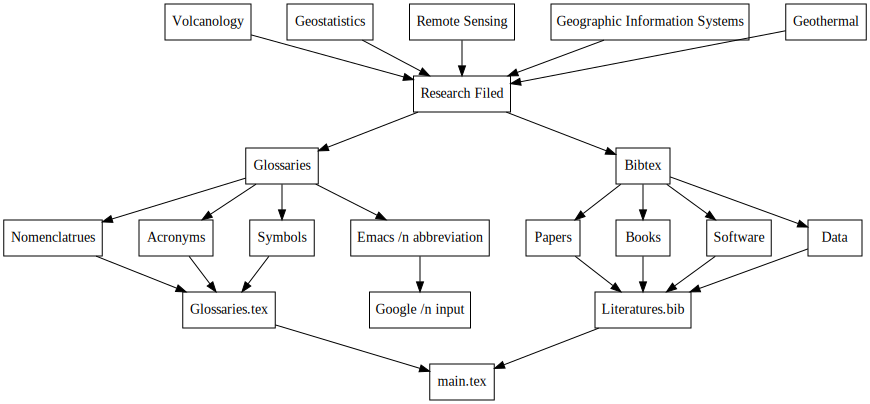
\includegraphics[width=.9\linewidth]{./glossaRWorkflow.pdf}
\section{fig:work with R to extract glossaries}
\label{sec-3}
\begin{verbatim}
digraph { 
fontname="Times"; 
fontsize = 12; 
splines = false; 
ranksep = 0.2; 
nodesep = 0.5; 
node [shape = box] 
//1. set node 
gls [label = "Glossaries"]
nomencl[label = "Nomenclatrues"]
acro [label = "Acronyms"]
symbol [label = "Symbols"]
xml [label = "XML", shape = circle]
df0 [label = "data.frame \n (raw)", color = blue]
df1 [label = "data.frame \n (unduplicated)", color = blue]
df2 [label = "data.frame \n (latex)",color = blue]
orgTable0 [label = "org table \n (raw) "]
orgTable1 [label = "org table \n (unduplicated)"]
orgTable2 [label = "org table \n (latex)"]
glsfile [label = "Glossaries.tex \n( keep Update)", color = red, fill=gray]
//2. set path 
gls -> {acro, nomencl, symbol} -> xml
xml -> df0 [label = " web scrape"]
xml -> orgTable0 [label = " paste \n& convert"]
df0 -> orgTable0 [label = " R:print"]
orgTable0 -> df1 [label = " R:!duplicate(df) \l babel:var"]
orgTable1 -> df1 [label = " R:print", dir = back]
orgTable1 -> orgTable2 [label = " unique Label \n format Latex \n remove Error"]
orgTable2 -> df2 [label = ":var "]
df2 -> glsfile [label= " paste\n write.table", weight = 10]
//3. set rank 
{rank = same; df0, orgTable0} 
{rank = same; df1, orgTable1} 
{rank = same; df2, orgTable2} 
}
\end{verbatim}

\includesvg[width=.9\linewidth]{orgAndR}

\section{R:}
\label{sec-4}

\section{tbl:Restec}
\label{sec-5}
\begin{verbatim}
###############################################################################
## R code chunk:
###############################################################################
\end{verbatim}
\section{Remote Sensing Glossaries}
\label{sec-6}

\subsection{\url{http://www.ldeo.columbia.edu/res/fac/rsvlab/glossary.html}}
\label{sec-6-1}
\begin{verbatim}
###############################################################################
## R code chunk:
###############################################################################
\end{verbatim}
Emacs 24.3.1 (Org mode 8.2.10)
\end{document}